% vim: tw=80

\chapter{The CMS Detector at the Large Hadron Collider}

The European Organization for Nuclear Research (CERN) was founded in 1954.
Originally dedicated to the study of atomic nuclei, it is now devoted to
study sub-atomic particles and their interactions. To accomplish that task, CERN
built several particle accelerators reaching record-breakign energies and
explored energy ranges not been accessible before.

Ground-breaking achievements like the discovery of neutral currents in the
Gargamelle bubble chamber, the discovery of the W and Z boson by the UA1 and UA2
experiments at the LEP accelerator or the creation of antihydrogen atoms were
made by physicists at CERN.

The LEP and Tevatron experiments have provided remarkabable insights into the
Standard Model and performed precision tests of the Standard Model. As a logical
consequence of the unsuccessfull search for the higgs boson in their energy
range, a even larger and more powerful accelerator was planned and built, the
Large Hadron Collider (LHC). The search for the higgs boson finally succeded in
2012, but many further question like the search for supersymmetry or dark matter
still need to resolved in the future.

\section{The Large Hadron Collider}

The Large Hadron Collider (LHC) is the world's most powerful particle
accelerator and collider. The LHC is contained in the circular tunnel of the
preceding Large Electron Positron (LEP) collider which has a circumference of 27
km at a depth between 50 and 175 m. The tunnel crosses the border between
Switzerland and France at four points and two of the four main experiments are
located in France. 

Two adjacent beamlines that intersect at four interactions points contain the
particle beams travelling in opposite directions. More than 1000 dipole magnets,
generating a magnetic field of up to 8.3 T bend the proton beams on the circular track while
almost 400 quadrupole magnets keep the beams focused. 

The proton beams are brought to collision at four interaction points which house
the LHC experiments ALICE~\cite{ALICE}, ATLAS~\cite{ATLASa}, CMS and
LHCb~\cite{LHCb}. ALICE is designed to study the quark-gluon plasma produced by
colliding heavy ions, which resembles the initial state of the universe. LHCB is
precisely measuring the CP violation and the decay of B mesons. ATLAS and CMS,
general purpose detectors allowing a broad field of phycis studies, were built
to search and study the Higgs boson and physics models beyond the standard
model. Additionally precision measurements of standard model predictions and
parameters improve the current knowledge and the confidence of predictions of
the standard model.

Prior to the injection and acceleration of protons in the LHC, the particles
pass a series of consecutive acceleration steps succesively increasing their
energy. The linear particle accelerator (LINAC2) generates 50 MeV protons, that
are further accelerated in the Proton-Synchrotron (PS) to 26 GeV and
the Super-Proton-Synchrotron (SPS) up to an energy of \SI{450}{\giga
\electronvolt}. At last the proton beams are injected into the LHC ring and are
further accelerated up to peak design energy of 13 TeV. All these
pre-accelerators are not only used to feed the LHC, but also serve other physic
experiments as can be seen in Figure~\ref{fig:lhc_complex}.

\begin{figure}[htp]
    \centering
    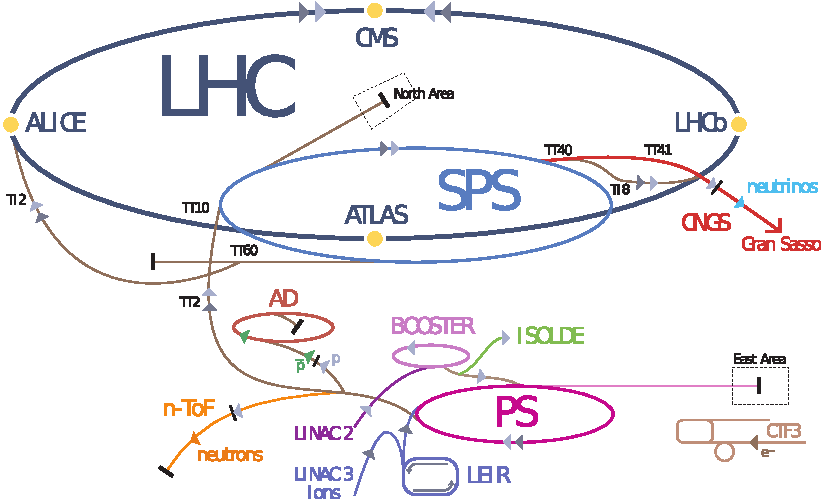
\includegraphics[width=0.8\textwidth]{figures/cms_detector/lhc_accelerator_chain.pdf}
    \caption[CERN accelerator complex]{Schematic view of the CERN
        accelerator complex. It shows the LHC ring  with the four beam crossing
        points as well as the various pre-accelerators~\cite{LHC:COMPLEX}.}
    \label{fig:lhc_complex}
\end{figure}

\subsection{The Compact Muon Solenoid Detector}

The Compact Muon Solenoid (CMS) detector is a general purpose detector at the
LHC, located at Point 5 of the LHC ring. To serve a wide range of physics
studies, the detector design is driven by a cylyndrical structure containing
layers of different subdetectors each built to measure a specific type of
particles with best precision. A high-precision inner tracking system is
surrounded by an electromagnetic and a hadronic calorimeter which again are
enclosed by a superconducting solenoid magnet. The whole inner part of the
detector is surrounded by a sophisticated muon detection system embedded in a
iron yoke. The detector is \SI{21.6}{\meter} long and \SI{14.6}{\meter} in
diameter, but weighing more than \SI{12000}{\tonne} due to its compact design.
It was built as cylyndrical slices constructed at ground level and lowered into
the cavern. In case of upgrades or repairs, the slices can be pulled apart and
the inner components can be easily accessed.

\begin{figure}[htp]
    \centering
    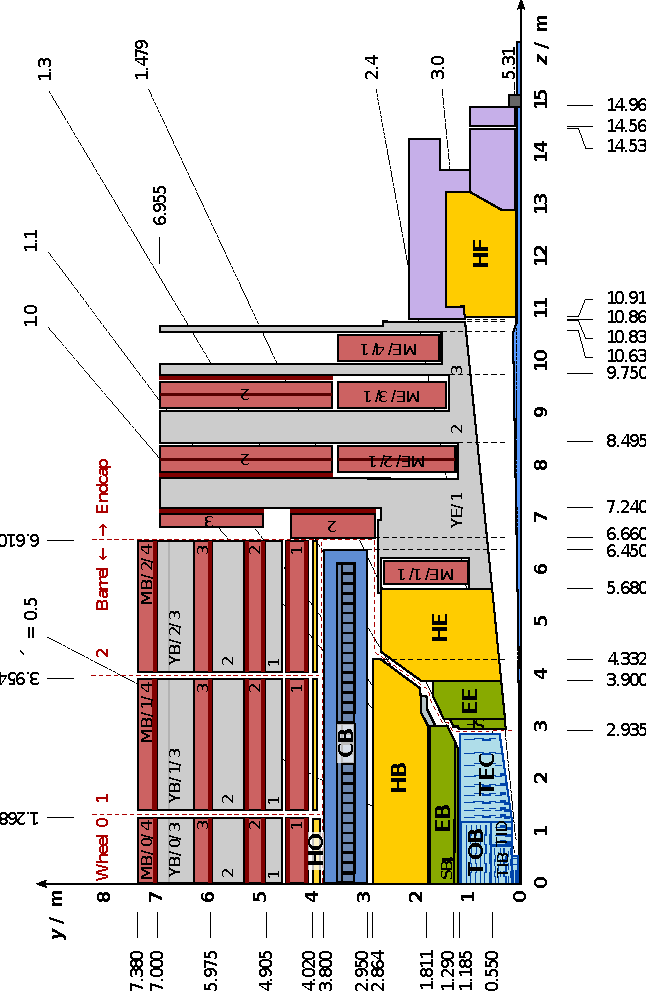
\includegraphics[width=0.8\textwidth]{figures/cms_detector/cms_longitudinal_section.pdf}
    \caption[Longitudinal section of the CMS
    detector]{A longitudinal section of one quadrant of the CMS
        detector in the $y$-$z$ plane. The sketch shows
    the multi-layer design of the CMS detector starting with the silicon pixel
and silicon strip detectors close to the interaction point. They are surrounded
by the electromagnetic (green) and hadronic (yellow) calorimeters. The barrel is
encompassed by the superconducting magnet (blue). The muon detection system
(red) is embedded in the iron return yoke~\cite{Berger:2014aca}.}
    \label{fig:cms:longitudinal_section}
\end{figure}

\todo{high requirements like 25 ns between collisions, high radiation level,
advanced detector materials.}

\subsection{Definition of the Coordinate System}

CMS uses a right-handed coordinate system centered at the nominal interaction point inside the
detector. The $x$-axis points radially inward towards the LHC ring centre, the
$y$-axis vertically upwards and the $z$-axis along the beam direction towards
the Jura mountains. Important quantities are the azimuthal angle $\phi$
measured from the $x$-axis in the $x$-$y$ plane and the polar angle $\theta$,
measured from the $z$-axis in the $z$-$y$ plane. Instead of the polar angle
$\theta$, the pseudo-rapidity $\eta$ and the rapidity $y$ are commonly used to
split the phasespace, since the differential flux is approximately constant at
hadron-hadron colliders. The pseudo-rapidity is defined as

\begin{equation*}
    \eta = - \ln \left( \tan \left( \frac{\theta}{2} \right) \right)
\end{equation*}

Throughout this thesis the rapidity is favoured compared to the pseudo-rapidity
due to its invariance under longitudinal boosts in the $z$-direction. Rapidity
and pseudo-rapidity are equivalent in the case of massless particles. The
rapidity is defined as

\begin{equation*}
    y = \frac{1}{2} \ln \left( \frac{E + p_z}{E - p_z} \right) 
\end{equation*}

The momentum along the beamline is not well defined due to the momentum
distribution inside the proton. A direct connection to the hard process is given
by the transverse momentum \pt related to cartesian coordinates as

\begin{equation*}
    \pt = \sqrt{p_x^2 + p_y^2}
\end{equation*}

\subsection{Inner Tracking System}
\todo{measurement of charged particles.}

To yield a best possible spatial resolution, the particle tracks need to be
measured as close to the beam line as possible. The inner tracking system of CMS
is designed to measure the tracks of charged particles emerging from the
collision. Enclosing the interaction point with a diameter of 2.6 m and
extending 2.8 m in each direction along the beampipe, the tracking system covers a
pseudo-rapidity range up to $|\eta| < 2.4$. The inner tracking system comprises
two subsystems, the silicon pixel detector consisting of three layers and
installed very close to the beam pipe and the silicon strip detector with ten
strip layers in the barrel region. 

\paragraph{Silicon Pixel Detector} Containing over \SI{65} milion pixels
arranged in three cylindrical layers at \SI{4}{\centi\meter},
\SI{7}{\centi\meter} and \SI{11}{\centi\meter} distance to the beam pipe, the
pixel detector is able to resolve the tracks of the huge number particles. At
LHC design luminosity, about 1000 particles pass the tracking detector on
average. The size of each pixel is \SI{100}{\micro \meter} x \SI{150}{\micro
\meter} giving a average occupancy of $10^{-4}$ per bunch crossing.  The high
spatial resolution achieved by the pixel detector additionally allows the
identification and measurement of secondary vertices used to identify long-lived
particles.

\paragraph{Silicon Strip Detector} The pixel detector is complemented by silicon
strip detector. Reduced particle flux further away from the beam pipe eases the identification
of tracks. Cost-efficient silicon strips are employed reaching out to
an radius of \SI{1.3}{\meter}. The strip detector consists of a total of 10 million
detecting strips read out by \SI{80000} chips. 

\begin{figure}[htp]
    \centering
    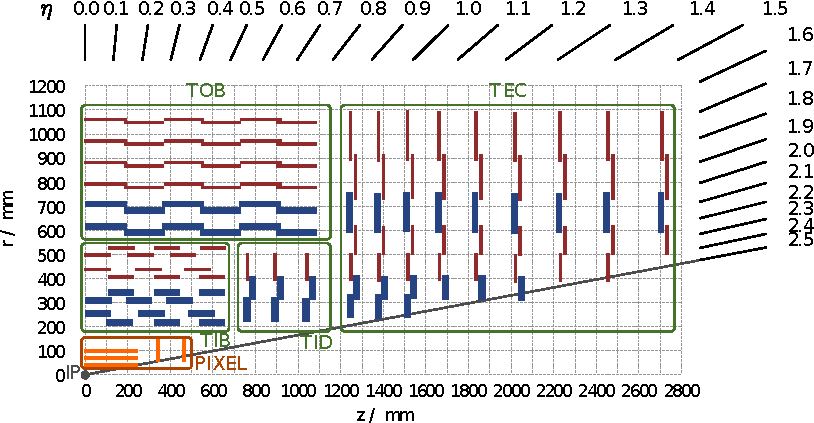
\includegraphics[width=0.65\textwidth]{figures/cms_detector/tracker.pdf}\hfill
    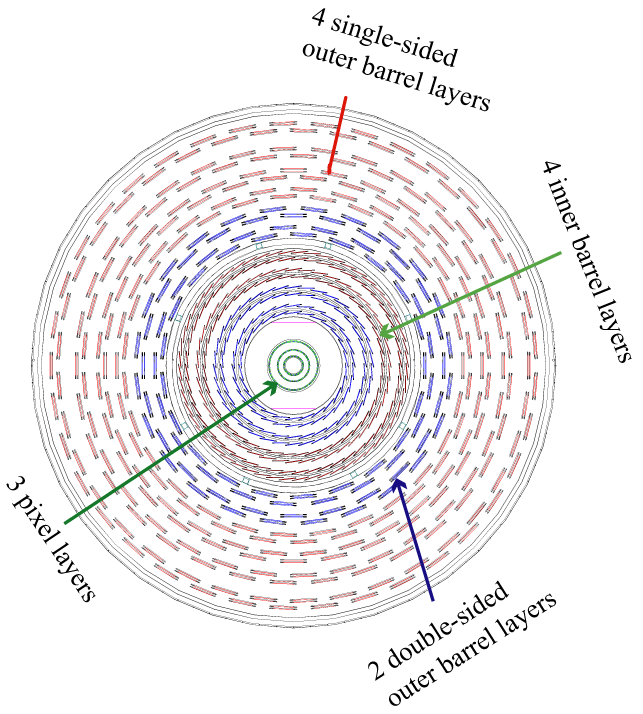
\includegraphics[width=0.3\textwidth]{figures/cms_detector/tracking_sytem_barrel_slice.png}
    \caption[Inner Tracking System]{The left figure shows one quadrant of the
        longitudinal section of the inner tracking system of CMS consisting of the
        silicon pixel detector and the silicon strip detector. The right figure shows a
        transverse section of the tracking system in the barrel region with overlapping
        arrangement of the strip modules. Figures from~\cite{Berger:2014aca} and
        \cite{cmsweb:innertracker}.}
    \label{fig:cms:inner_tracking}
\end{figure}

\subsection{Electromagnetic Calorimeter}

Measuring the track of the traversing particles is not sufficient to derive to
measure the momentum. The energy needs to be measured by stopping the particles
in the detector and measuring the size of the deposited energy. The photon and
electron energy is measured in the electromagnetic calorimeter (ECAL). 

High-energetic photons, electrons or positrons which enter the dense material of the ECAL
detector, produce an electromagnetic shower via subsequent bremsstrahlung and
electron-pair production processes. Below a certain threshold, the particles
deposit their energy via compton scattering and the photo-electric effect in the
detector material resulting in an excitation of their atomic state. When they
return to the ground state, they emit photons, which can be measured using
avalanche photodiodes. The fraction of the deposited energy is to the number of
emitted photons.

The hermetic calorimeter is made of lead tungstate ($\mathrm{PbWO}_4$), a very
dense material with a radiation length of $X_0 = 0.89$ cm. Through the
additional oxygen, it is a highly transparent and scintillates light. These
material properties allow the calorimeter to be built very compact within the
solenoid magnet. Additionally, the small Moli`ere  radius of 2.19 cm leads to a
fine granularity. 

\begin{figure}[htp]
    \centering
    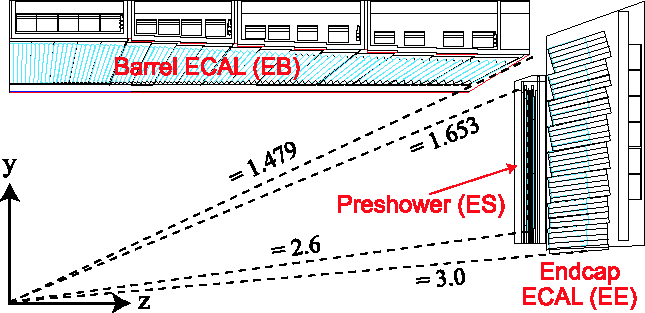
\includegraphics[width=0.8\textwidth]{figures/cms_detector/cms_ecal.pdf}\hfill
    \caption[Electromagnetic Calorimeter]{The electromagnetic calorimeter
    consists of two submodules covering the barrel regiond and the endcaps.
    Additionally a preshower detector is mounted in front of the
    endcaps~\cite{cms:ecal}.}
    \label{fig:cms:ecal}
\end{figure}

Figure~\ref{fig:cms:ecal} shows a schematic sketch of the ECAL in the $y$-$z$
plane. The ECAL consists of three subsystems covering the the pseudo-rapidity
range upt to 3.0. The \textbf{electromagnetic calorimeter barrel (EB)} covers up
to $\eta < 1.479$ using more than 60000 crystals forming a homogenous coverage
in pseudo-rapidity. Each crystal measures 2.2 cm x 2.2 cm x 23 cm corresponding
to a radiation length of 25.8 $X_0$. The \textbf{electromagnetic calorimeter
endcaps (EE)} extend the pseudo rapidity coverage from $1.479 < |\eta| < 3.0$.
The largest part of the ECAL endcap is additionally covered by the
\textbf{electromagnetic pre-shower detector (ES)}. It consists of two orthogonal
silicon strip sensors. The ES improves the discrimination between single
high-energetic photos and less interesting low-energy photon pairs as well as
the discrimination between neutral pions and photons.

The relative energy resolution of the ECAL can be parametrized using the NSC-formula

\begin{equation}
    \left( \frac{\sigma}{E} \right)^2 = \frac{N^2}{E^2} + \frac{S^2}{E} + C^2
\end{equation}

in which the first term describes the contribution by noise (N), the second
term the stochastic (S) component arising from the proportional relation between
the number of counted photons and the deposited energy and last a constant (C)
term.

\subsection{Hadronic Calorimeter}

The compact design of the CMS detector limits the size of the calorimeters. CMS
therefore built a sampling calorimeter inside the solenoid coil. The hadronic
calorimeter consists of brass as absorber material which is non-magnetic and
has a short interaction lenth of $\lambda_I = 16 \si{\centi\metre}$. It is
interleaved with plastic scintillators measuring the deposited energy. The CMS
hadronic calorimeter comprises three subsystems. The \textbf{Hadron Barrel
Calorimeter (HB)} covers the barrel region up to a pseudo-rapidity $|\eta| <
1.305$. The absorbing material in the barrel has a corresponding thickness of
$5.39 \lambda$ in the central region up to $10.3 \lambda$ at $|\eta| = 1.3$. The
HB is complemented by the \textbf{Hadron Outer Calorimeter (HO)} located on top
of the coil of the magnet. Using the coil as absorbing material it is able to
meaure the tails of hadron showers penetrating the HB and the coil.The
\textbf{Hadron Endcap Calorimeter (HE)} extends the pseudo-rapidity coverage up
to $|\eta| < 3.0$. A major challenge in the construction of the HE were the
usage of non-magnetic material to not disturb the magnetic field as well as the
close distance to the beampipe. Radiation damages decrease the detector response
and have to be corrected for continously. The \textbf{Hadron Forward (HF)}
calorimeter extends even closer to the beam pipe. With a coverage of $2.8 <
|\eta| < 5.2$ the calorimeter is adapted to the high radiation environment. The
HF is desinged using iron absorbers and quartz fibres as active material, which
measure the Cerenkov light emitted by the relativistic components of the
shower.

Hadrons entering the calorimeter produce a hadronice shower. High-energetic
hadrons mostly shower in inelatic interactions producing a large number of pions
and nucleans. Due to the large transverse momentum of these secondary particles,
hadronic shower spread further in the calorimeter than electromagnetic shower.
When the energy of the particles involved in the shower drops below a certain
theshold, the energy is deposited by ionisation and low-energy hadronic
activity. The active scintillation material is excitated eand emits blue-violet
light. The scintillators are connected to photodiodes using wavelength
shifters which read out the signals and pass it to the data aquisition system.

\subsection{Superconducting Solenoid}

A key component of the CMS detector is the superconductiong magnet which
produces a magnetic field of 4 T and is located inside the detector between the
calorimeters and the muon system. It measures a diameter of 6 m and a lenth of
12.5 m. When operated at design magnetic field strenth, the magnet contains an
energy of 2.6 GJ. The strong magnetic field is neccessary to bend the particle
tracks for a high momentum resolution in the tracking system. Operated at a
temperature of 4 K, the NbTi conductors become superconducting. The muon system
is installed within a 10,000 t iron yoke which return the magnetic field.

\subsection{Muon System}

Identifying and measuring muons with high precision is an unrivalled capacity of
the CMS detector. Unlike most other particles, muons are not stopped by the
calorimeters but leave the detector. Therefore, the muon system has been placed
around the other detector components to measure the bended tracks of the muons.

By combining the information of the inner tracking system and the muon
detectors, the path and the muon momentum can be measured precisely. The muon
system comprises three different types of detectors each suited for a specific
task. Drift tubes (DT) cover the barrel region up to $\eta < 1.2$, the endcaps
up to $\eta < 2.4$ are measured using cathode strip chambers (CSC) which also
work reliably in spatially varying magnetic field. The DT and CSC detectors
yield a precise spatial muon resolution. Both system are accompanied by
resistive plate chambers (RPC) which provide a fast response to the trigger
system.

\subsection{Trigger and Data Aquisition at CMS}

The LHC generates a huge number of collisions. At a beam crossing frequency of
25 ns, there are 40 million bunch crossings per second with an average of around
20 collisions per bunch crossing. With todays available hardware, the storage of
all collision data is not possible. Furthermore, most of the collisions are soft
and of low interest for physics analyses. Therefore a complex trigger system
consisting of a very fast hardware implemented component, the Level 1 trigger
(L1) and a software trigger, the High Level Trigger (HLT), analyses the incoming
data and decides if a collision event is of interest and should be stored
permanently or is omitted.

\begin{figure}[htp]
    \centering
    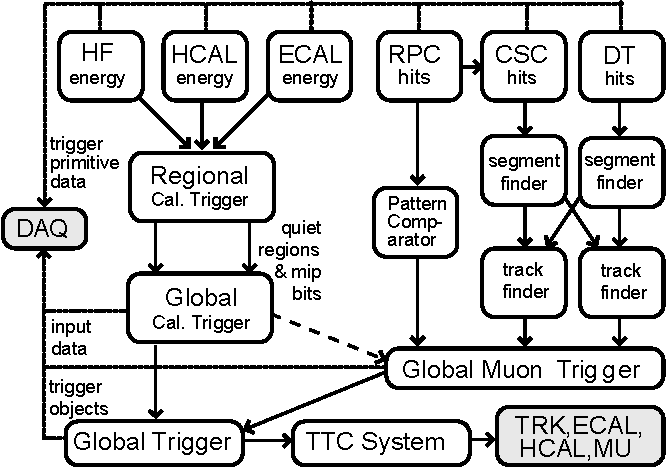
\includegraphics[width=0.8\textwidth]{figures/cms_detector/cms_l1_trigger.pdf}\hfill
    \caption[The L1 Trigger of CMS]{asdf\cite{Sphicas:2002gg}}
    \label{fig:cms:l1_trigger}
\end{figure}

When a collision occurs, the detector electronics is readout and directly
analyzed using custom hardware, the \textbf{L1 trigger}. Of special interest for
this thesis are the calorimeter triggers. Figure~\ref{fig:cms:l1_trigger} shows
the workflow of the L1. The Trigger Primitive Generators convert the frontend
electronics readout into transverse energy. The Regional Calorimeter Triggers
(RCT) identify electromagnetic shower in the ECAL and sum up the ECAL and HCAL
trigger tower. Additonally a patter recognition is performed to identify jets
and hadronic $\tau$ decays. These candidates are then passed to the Global
Calorimeter Trigger which sorts the incoming candidates from the all 18 regional
triggers and passes the top canadites to the Global Trigger (GT). If the global
trigger accepts the event it is further processed by the data aqusition system
and passed to the high level trigger.

the \textbf{High Level Trigger} is fully implemented in software running on a
dedicated computing farm at Point 5. The software is implemented in the CMS
reconstruction software and can therefore access all information from the whole
detector as well as aplly basic jet energy corrections. Jet Trigger for example
need to pass a \pt threshold on reconstructed calorimeter jets before complex
particle flow and jet reconstruction algorithm are performed to save processing
time.

The data aquisition system can apply prescales on each trigger to reduce the
rate at which a trigger fires. Especially for single jet triggers, which
trigger on the jet \pt, need to be prescaled in the low-\pt region to avoid huge
rates. Of course the trigger prescales have to be taken into account again when
the spectrum is reconstructed from the number of events.

The DAQ system assembles the events which it receives from the L1 trigger at a
rate of 100 kHz.

\begin{figure}[htp]
    \centering
    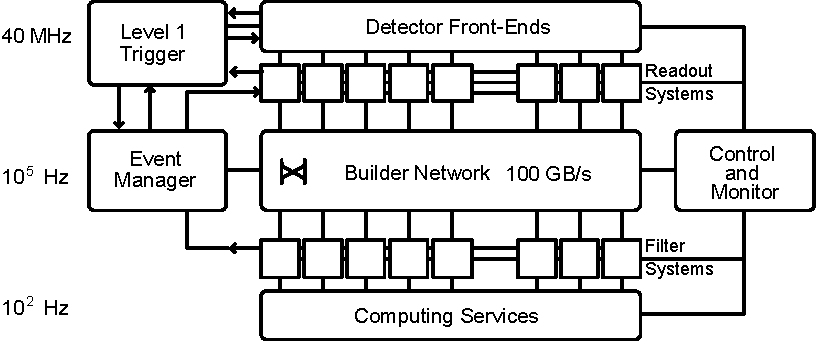
\includegraphics[width=0.8\textwidth]{figures/cms_detector/cms_daq.pdf}\hfill
    \caption[The DAQ System of CMS]{asdf~\cite{Sphicas:2002gg}}
    \label{fig:cms:daq_system}
\end{figure}

The event rate is reduced by the L1 trigger to 100 kHz. The DAQ system then
reads out the data of all detector components and assembles the complete events
at this rates, see Figure~\ref{fig:cms:daq_system}. The data is then transferred
to the HLT computing farm in which the sophisticated software-based trigger further
reduces the event rate to a few hundred events per second. The passing events
are then merged by the storage managing system and written to the Tier-0
computing centre at CERN.

\section{Software and Computing Infrastructure}

The vast amount of and the complexity of the data produced at the LHC
experiments poses many challenges for the computing infrastructure and the
software. On the theory side, powerful Monte-Carlo event generators need to be
developed which are able to simulate the collision events. On the experimental
side, the raw detector the physical event information needs to be reconstructed. Additionally the
complex architecture of the detector response needs to be modelled and
simulated. These central tasks are approached using a common software framework
within CMS, the CMSSW framework, which interfaces the various theory tools and
all the reconstruction and detector software. All of these taks are divided
into smaller processing tasks, called jobs, which are assigned to computing
centers distributed over many countries. This common computing and storage
infrastructure is called the worldwide LHC computing grid (LHCG).

\subsection{CMS Software Framework}

The software framework of the CMS collaboration, referred to as CMSSW, offers
all neccessary tools for a phycis analysis. The tasks in the event processing
comprise on the one hand calibration and reconstruction of data from raw
detector read out and on the other hand the event generation and detector
simulation. Furthermore it provides the possibility to implement analysis code
to perform the data analysis. 

To cope with this vast range of requirements to the experiment software, CMSSW
is built on top of an event data model (EDM) in which the event is a
container for for all measured or simulated data. The reconstruction and
distribution algorithms in CMSSW are divided into modules, which can be
modularly loaded and run. Each module can read the event data and add additional
objects calculated within the algorithm. The execution of the modules is ordered
in processing chains which are configured by the user. Very often these modules
access external libraries like Monte Carlo event generators for event
simulation, Geant 4 for the detector simulation or FastJet for the
reconstruction of jets. Using this modular approach in which modules are loaded
dynamically one can easily start with an event containing only the raw detector
data and process all neccessary steps to arrive at the final event containing
the reconstructed objects suited for analysis.

While having that much information in the event data is convenient to redo
reconstruction steps, it is unsuited for fast processing in the analysis due to
its size and complexity. Therefore a skimming step, in which only the neccesary
data is preserved is run before the analysis, see Section~\ref{artus_kappa}.

\subsection{Analysis Software and Workflow}

Due to the complexity of the workflows in the HEP data analysis, several tools
were used or even deloped in the Karlsruhe group to faciliate a reliable and
fast workflow for the analysis. 

\subsubsection{Artus and Kappa}
\label{artus_kappa}

The Kappa software is a skimming framework interfaced to CMSSW. It consists of
different modules which allow to skim only the physics objects needed in the
subsequent analysis. The data is then stored in its own compact data format
using the ROOT format. The resulting Kappa tuples provide all neccesary
information of the events and the lumisection while hiding the complexity of the
CMSSW datasets. There is a separate tool collection, KappaTools, in which
functions to access the Jet energy corrections or HLT informations are
collected.

The analysis itself is built on top of the Artus framework. Artus was developed
within the Karlsruhe group to combine analysis efforts and profit from mutual
developments. The framework defines a workflow based on three elements. There
are \emph{producers}, which calculate quantities and \emph{filters}, which reject events based on
the defined criteria. In a final step, histograms or nTuples are written out by
\emph{consumers}. All producers, filters and consumers are written in a modular
way so that they can be shared with other analyses. Furthermore they are steered
by a global configuration file in which one can easily adapt all settings and
cuts.

\subsubsection{grid-control}

The data sets are even after the skimming step to large to be processed on a
single computer. Therefore special batch system with a huge number of computing
nodes are employed to process the data. The data processing is split into
multiple jobs which are then sent to the batch system. grid-control is by far
the most versatile job submission tool which provides multiple options for data
splitting and parametrized jobs while hiding the pitfalls of local or remote
computing resources.

\subsubsection{ROOT}

The object-oriented data analysis framework ROOT has been written almost 20 years
ago. It is used by all LHC experiments for persistent storage of data. Moreover
ith provides fast histogramming classes and access to many libraries like MINUIT
for minimization purposes or TMVA for multivariate data analyses. Despite
many hours of headaches caused by obscure design decisions in the software, ROOT
and especially the python bindings PyROOT were used extensively in this analysis.

\subsubsection{matplotlib and numpy}



\subsection{Monte-Carlo Event Generators and Simulation Software}
\label{subsection:mc_generators}

\subsubsection{Pythia}

The multi-purpose event generator Pythia simulates events in high-energy
collisons, comprising a large set of physics processes. Pythia uses the Lund
string hadronization model in which all but the highest-energy gluons are
treated as field ines which attract each other by gluon self-interaction and
form a tube or string of strong color field. In this analysis two version of the
Pythia event generator are used. The official samples including the detector
simulation were generated using Madgraph and Pythia 6, while the study of
non-perturbative effects was performed using the new Pythia 8 version, in which
all the new tunes were available. 

\subsubsection{Herwig}

Herwig is also a multi purpose event generator for the simulation of high-energy
hadron-hadron collisions. The first version was build in Fortran and is known as
HERWIG~\cite{Corcella:2000bw}. Herwig++~\cite{Bahr:2008pv} builds up on the
heritage of the HERWIG version while providing a much more flexible structure as
it is implemented in C++. The recently released Herwig 7~\cite{Bellm:2015jjp}
version combines all their developments and supersedes both version. 

The Herwig generator family includes all steps to simulate events. It includes a
number of hard scattering processes, but also possesses the possibility to
interface external matrix element generators. The parton shower simulates
initial- and final-state radiation via angular ordering, multiple partonic
scatterings are simulated by an eikonal model and a cluster model decribes the
hadronization. 

Herwig 7 further improves these capabilities by including next-to-leading order
QCD matrix elements with matched parton showers while keeping the key features
of the previous Herwig versions. Herwig++ is used in this thesis to study
non-perturbative effects, see Sec.~\ref{sec:np_factors}. The NLO capabilities of
Herwig 7 are shown in the comparison of the unfolded measurement to NLO
predictions with matched parton showers, see Sec.~\ref{sec:nlo_comparisons}.

\subsubsection{Madgraph}

\subsubsection{NLOJet++ and fastNLO}
\label{sec:nlojetpp}

% To populate the whole accessible phasespace with sufficient events to get a
% precise prediction, a huge number of events is neccessary. Since especially the
% influence of the PDFs and the strong coupling constant is interesting to be
% studied, the calculation would have to be repeated multiple times with different
% input parameters. In order to speed-up this process, \NLOJETPP is interfaced to
% the \fastNLO package~\cite{Kluge:2006xs,Britzger:2012bs}. fastNLO uses
% sophisticated interpolation tables to store the matrix element coefficients as a
% function of the scales, the calculation order and the fractional proton
% momentum. The fastNLO tables can now be evaluated with different PDFs, \as and
% scales within negligible time. 


The complicated NLO cross section for jet productions are calculated using
\NLOJETPP. It implements the dipole subtraction method for the separation of the
divergences. \NLOJETPP can calulate up to three-jet observables at NLO precision.
It implements the ability run analysis scenarios by which it is interfaced to
\fastNLO.

Since the pQCD cross section calculations in \NLOJETPP are determined in Monte
Carlo integration and are therefore very time consuming. For fits of the proton
structure or the extraction of the stroung coupling constant, the cross sections
need to be evaluated multiple times with different input parameters. The
\fastNLO framework implements a strategy for a fast recalculation of these cross
section. It sotres the perturbative coefficients obtained with \NLOJETPP in a
way that the strong coupling constant and the PDFs can be changed afterwards
without a recalculation of the perturbative coefficients.

\subsubsection{LHAPDF}

All event generators and cross section calculation tools need the parton
distribution functions as input. They are either hardcode in the generator or
accessed using a standardized interface, the LHAPDF library. LHAPDF provides
interpolation routines by which PDFs read from discretised data files can be
accessed. 
